\documentclass[11pt,letterpaper]{article}

\usepackage[margin=1in]{geometry}
\usepackage{times}
\usepackage{setspace}
\usepackage{graphicx}
\usepackage{booktabs}
\usepackage{tabularx}
\usepackage{amsmath,amssymb}
\usepackage{hyperref}
\usepackage{caption}
\usepackage{subcaption}
\usepackage{xcolor}
\usepackage{enumitem}
\usepackage[T1]{fontenc}
\usepackage[utf8]{inputenc}

\hypersetup{
  colorlinks=true,
  linkcolor=black,
  citecolor=black,
  urlcolor=blue
}

\graphicspath{{figures/}}
\onehalfspacing
\setlength{\parskip}{0.4em}

\title{\textbf{Fifteen Years of Housing Crisis in Canada, 2006--2021:\\
A High-School Research Paper Using Residual Income}}
\author{High School Research Paper\\[0.4em]
\large Draft Version 3.0}
\date{17 October 2026}

\begin{document}
\maketitle

\begin{abstract}
\noindent\textbf{Background.}
The usual 30\% shelter-cost-to-income rule can hide hardship.
A household may look ``affordable'' on paper and still not have enough money left for food, transport, or clothing.

\noindent\textbf{Objective.}
This paper asks how Canadian housing hardship changed from 2006 to 2021 when hardship is defined by leftover income, not by the 30\% rule.

\noindent\textbf{Methods.}
We analysed 777,707 valid person-records from the Census 2006, 2011, and 2021 Public Use Microdata Files.
These are unweighted hierarchical person-records, not household totals and not survey-weighted estimates.
Residual income equals after-tax income minus annual shelter cost.
Housing hardship is flagged when residual income falls below a single-adult national Market Basket Measure leftover line, not the official region- and family-size MBM.
All dollars are converted to 2021 constant CAD.
Census 2016 is excluded because only 9.4\% of records survived cleaning.

\noindent\textbf{Results.}
Over 15 years, inflation-adjusted median shelter costs rose 37.1\% while median income rose 33.5\%.
Hardship stayed high: 38.0\% in 2006, 33.9\% in 2011, and 37.9\% in 2021.
Renters had higher hardship than owners, but both groups worsened after 2011.

\noindent\textbf{Conclusions.}
The housing squeeze is structural, not a short recession effect.
It survived recovery, three federal governments, and COVID-19.
Policies that only watch the 30\% rule will miss the households that cut food and other basics to keep rent paid.

\medskip
\noindent\textit{Keywords:} housing affordability; residual income; Market Basket Measure; Census PUMF; Canada
\end{abstract}

\tableofcontents
\newpage

%% ====================================================================
\section{Introduction}
\label{sec:intro}

\subsection{The problem}
\label{sec:problem}

Canada has a housing affordability problem that has lasted more than a decade.
Many families pay rent or a mortgage and then do not have enough left for food, transport, a phone, or clothes.
That problem matters for students who want to move out, go to university, or save for a first home.

The common school and policy rule is the \textbf{30\% rule}: housing is ``affordable'' if it costs less than 30\% of income.
That rule is easy to calculate, but it is incomplete.
A household spending 28\% of income on rent can look fine and still have almost nothing left for groceries.

\subsection{A better measure: residual income}
\label{sec:ri}

Canada Mortgage and Housing Corporation (CMHC) uses a leftover-income test \cite{cmhc2024}.
Ask: after housing is paid, is there enough money left to buy a basic basket of non-housing needs?

\begin{align}
\text{Annual shelter cost} &= 12 \times \text{monthly shelter cost} \label{eq:shelter} \\
\text{Residual income} &= \text{after-tax income} - \text{annual shelter cost} \label{eq:ri} \\
\text{Hardship} &= 1 \text{ if residual income} < \text{MBM poverty line} \label{eq:hard}
\end{align}

The Market Basket Measure (MBM) is Canada's official poverty line for that leftover basket (food, clothing, transport, and other basics, excluding housing) \cite{statcan2021mbm}.

\subsection{Why fifteen years?}
\label{sec:why15}

A one-year snapshot cannot tell a temporary shock from a built-in problem.
Three Census waves cover:
\begin{itemize}[leftmargin=1.4em]
  \item \textbf{2006--2011:} the 2008 financial crisis and recovery;
  \item \textbf{2011--2016:} low-rate expansion (2016 data are too incomplete to use);
  \item \textbf{2016--2021:} the late-2010s housing peak and COVID-19.
\end{itemize}
If hardship falls when the economy is strong, the crisis is cyclical.
If hardship stays high through recovery, it is structural.

\subsection{Research questions}
\label{sec:rq}

\begin{enumerate}[leftmargin=1.6em]
  \item How did residual-income housing hardship change in Canada from 2006 to 2021?
  \item Which interval---2006--2011 or 2011--2021---was worse for leftover income?
  \item Did the owner--renter hardship gap widen, shrink, or stay the same?
\end{enumerate}

%% ====================================================================
\section{Methods}
\label{sec:methods}

\subsection{Data sources}
\label{sec:data}

\subsubsection{Census Public Use Microdata Files}

We used three Statistics Canada hierarchical PUMF files \cite{statcan2022pumf}.
Hierarchical files are \textbf{person records} nested in households.
This draft treats each cleaned person-record as the unit of analysis.
It does \emph{not} collapse income to the household and does \emph{not} apply the PUMF sampling weight (\texttt{WEIGHT}).

\begin{itemize}[leftmargin=1.4em]
  \item \textbf{Census 2006} (catalogue 95M0029X hierarchical): 78,056 valid records after cleaning (23.4\% of the raw file).
  \item \textbf{2011 National Household Survey} (catalogue 99M0002X hierarchical): 341,030 valid records (99.3\%). This wave is a voluntary survey, not a Census long form.
  \item \textbf{Census 2021} (\texttt{98M0001X2021002}): 358,621 valid records (99.1\%).
\end{itemize}

\textbf{Total analytical sample:} 777,707 person-records.

Census 2016 was downloaded and inspected, then dropped.
After the same missing-code rules, only 29,056 records (9.4\%) remained, and medians were not comparable (median income \$20,558; median shelter \$649).
Those values are data-quality artefacts, not a real 2016 collapse.
Shelter cost is \texttt{GROSRT} (gross rent) on the pre-2016 files used here and \texttt{SHELCO} (unified shelter cost) on 2021.
Those concepts are related but not a fully harmonized shelter series.
Owner's major payments (\texttt{OMP}) were not used, so 2006 owner hardship could not be estimated.

\subsubsection{Market Basket Measure thresholds}

Year-specific national-average leftover lines for a \textbf{single adult} were:
\begin{itemize}[leftmargin=1.4em]
  \item 2006: \$13,500
  \item 2011: \$15,000
  \item 2021: \$19,728
\end{itemize}
These are \emph{not} Statistics Canada's official region- and family-size MBM thresholds (catalogue 75F0002M).
They are a simplified national leftover basket used so that three waves can be compared with one rule.
A large family in Toronto and a single adult in a smaller city are judged against the same dollar line.
That is a real limitation, not a rounding detail.

\subsection{Variable construction}
\label{sec:vars}

\subsubsection{Inflation adjustment}

All money values are in 2021 constant dollars using CPI:
\begin{itemize}[leftmargin=1.4em]
  \item 2006 dollars $\times$ 1.276
  \item 2011 dollars $\times$ 1.148
  \item 2021 dollars $\times$ 1.000
\end{itemize}
Example: \$1,000 of 2006 rent equals \$1,276 in 2021 dollars.

\subsubsection{Housing hardship (primary outcome)}

Hardship follows Equations~\eqref{eq:shelter}--\eqref{eq:hard}.
This is the CMHC residual-income (V2) framework.

\subsubsection{Shelter-cost-to-income ratio (comparison measure)}

\[
\text{STIR} = \frac{12 \times \text{monthly shelter cost}}{\text{annual income}}.
\]
STIR $>$ 30\% is the usual ``affordability burden.''
STIR $>$ 50\% is ``severe burden.''

\subsubsection{Tenure}

Owners occupy a dwelling they own (with or without a mortgage).
Renters occupy a rented dwelling.
Owner hardship could not be estimated for 2006 after cleaning.

\subsection{Data cleaning}
\label{sec:clean}

PUMF files mark missing or not-applicable values with 8888, 9999, and 99999.
Those codes were set to missing.
A record was kept only if:
\begin{enumerate}[leftmargin=1.6em]
  \item annual income $> 0$;
  \item monthly shelter cost $> 0$ and $< \$10{,}000$;
  \item key fields were not missing.
\end{enumerate}
The 2006 file kept far fewer records than 2011 or 2021, so 2006 results should be read with extra caution.

\subsection{Statistical analysis}
\label{sec:stats}

For each year we report:
\begin{itemize}[leftmargin=1.4em]
  \item median and quartile income and shelter cost (2021 CAD);
  \item STIR $>$ 30\% and STIR $>$ 50\%;
  \item residual-income hardship rate and count;
  \item hardship by tenure where tenure is available.
\end{itemize}
We then compute percent changes in medians and percentage-point changes in rates.
We report medians, not means, because hierarchical PUMF files produce inflated household-level means when special income codes are left in the average.
Rates are unweighted shares of valid person-records.

Five figures and five tables were saved as separate files (see Appendices~\ref{app:figures} and~\ref{app:tables}) and included below with \texttt{\textbackslash includegraphics} and \texttt{\textbackslash input}.

\subsection{Ethics}
\label{sec:ethics}

The analysis uses public, anonymized PUMF files.
No ethics review is required under Statistics Canada PUMF rules.
No household can be identified from these files.

%% ====================================================================
\section{Results}
\label{sec:results}

\subsection{Sample characteristics}
\label{sec:sample}

\begin{table}[htbp]
\centering
\caption{Sample characteristics by Census year (inflation-adjusted to 2021 CAD)}
\label{tab:sample}
\small
\begin{tabular}{lrrr}
\toprule
Characteristic & 2006 & 2011 & 2021 \\
\midrule
Valid sample size ($n$) & 78,056 & 341,030 & 358,621 \\
Median income (2021 CAD) & \$34,452 & \$45,920 & \$46,000 \\
Income 25th percentile & \$17,864 & \$22,960 & \$25,000 \\
Income 75th percentile & \$70,180 & \$101,024 & \$93,000 \\
Median monthly shelter & \$1,021 & \$1,378 & \$1,400 \\
Shelter 25th percentile & \$766 & \$804 & \$800 \\
Shelter 75th percentile & \$1,531 & \$2,181 & \$2,129 \\
STIR $>$ 30\% & 57.0\% & 52.2\% & 50.8\% \\
STIR $>$ 50\% & 35.8\% & 33.6\% & 31.5\% \\
Housing hardship rate & 38.0\% & 33.9\% & 37.9\% \\
Households in hardship ($n$) & 29,681 & 115,459 & 135,740 \\
\bottomrule
\end{tabular}
\par\smallskip{\footnotesize Notes: All dollar values converted to 2021 constant dollars using CPI multipliers (2006 $\times$ 1.276; 2011 $\times$ 1.148). Census 2016 is excluded because valid-record retention was 9.4\%. Estimates are unweighted person-records from hierarchical PUMF files. Median income is reported instead of the mean because hierarchical PUMF files produce inflated household-level means.}
\end{table}


The 2021 median income is \$46,000 (2021 CAD).
The 2021 median monthly shelter cost is \$1,400.
The interquartile range for shelter stays wide: about \$800 to \$2,100.

\subsection{Fifteen-year national trends}
\label{sec:trends}

\begin{figure}[htbp]
  \centering
  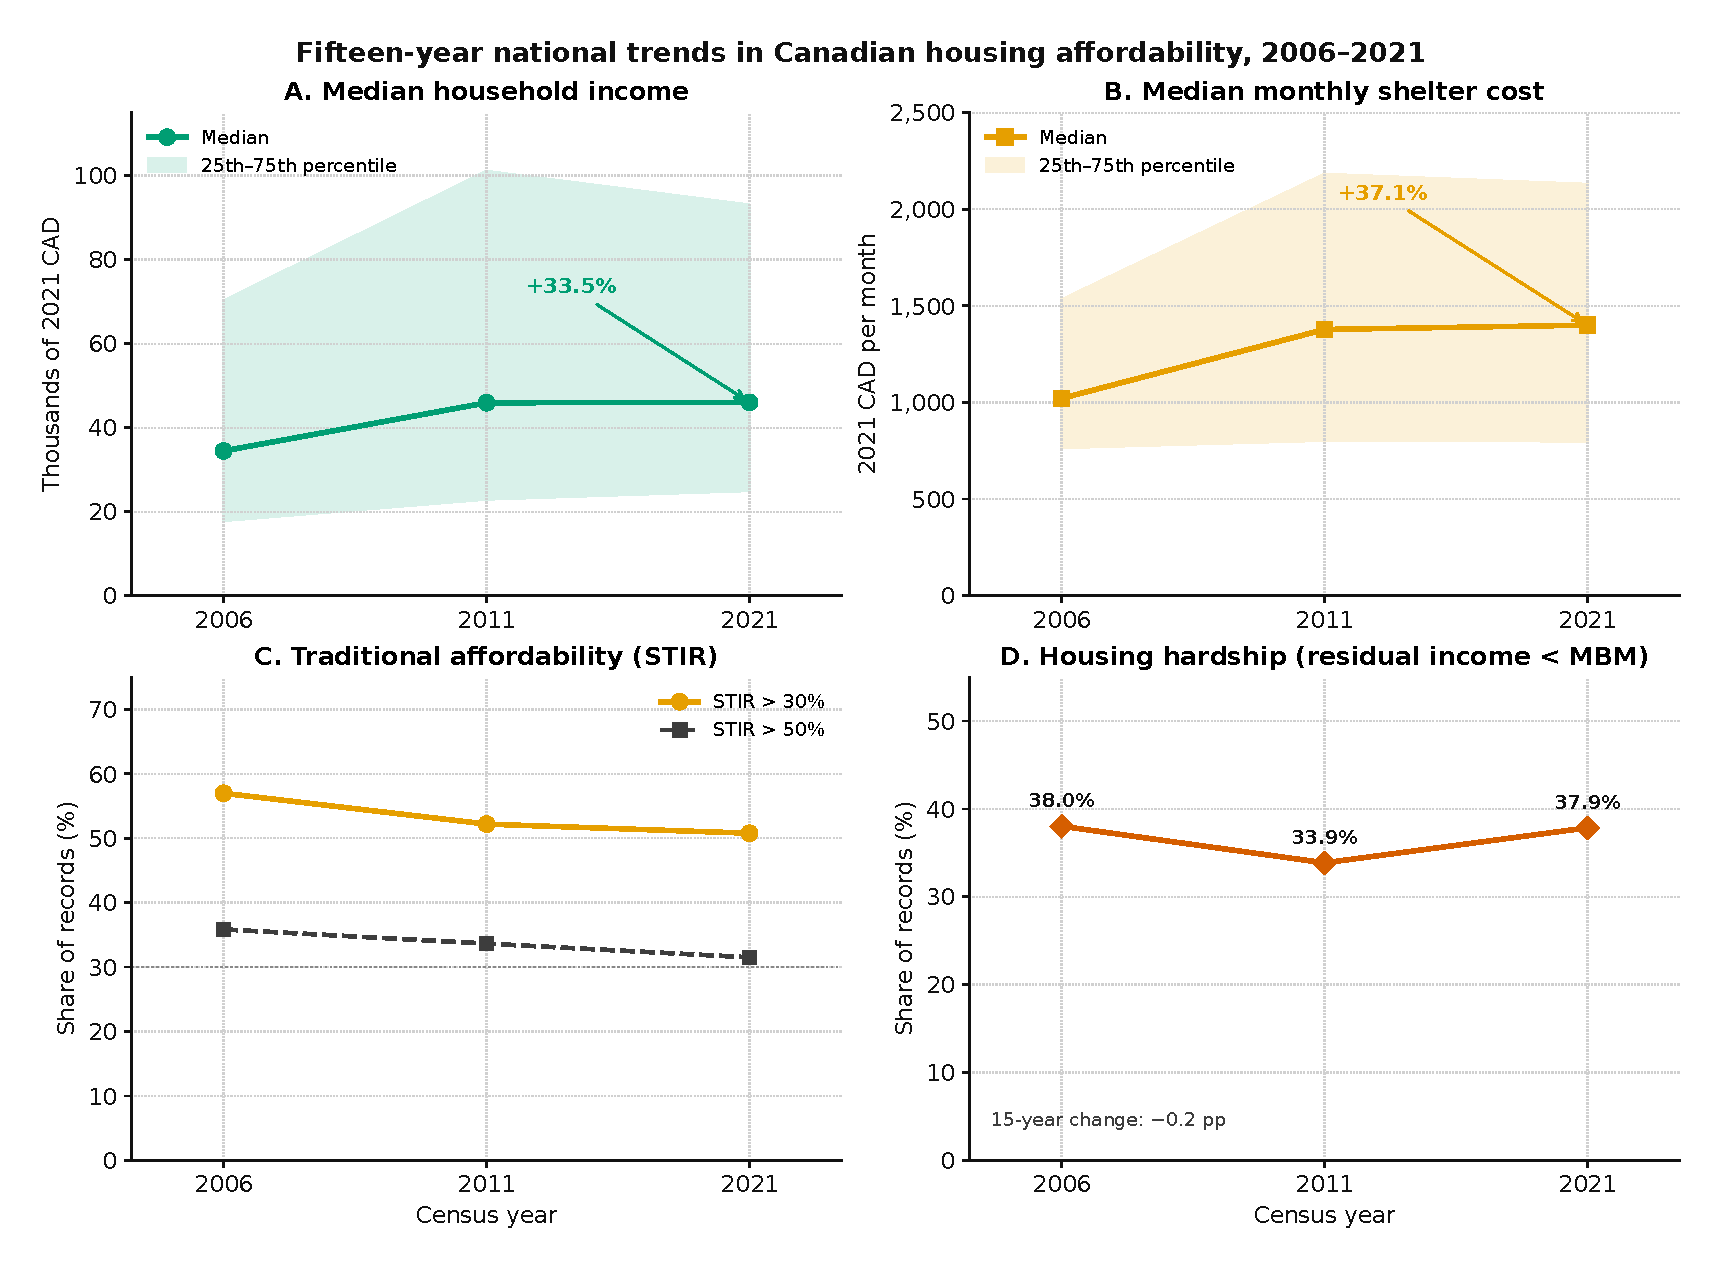
\includegraphics[width=\textwidth]{fig01_national_trends.pdf}
  \caption{Fifteen-year national trends, 2006--2021.
  Panel~A: inflation-adjusted median income with the 25th--75th percentile band.
  Panel~B: inflation-adjusted median monthly shelter cost with the same band.
  Panel~C: traditional STIR shares.
  Panel~D: residual-income housing hardship.
  Census 2016 is omitted (see Section~\ref{sec:data}).}
  \label{fig:national}
\end{figure}

\textbf{Income.}
Median income rose from \$34,452 (2006) to \$46,000 (2021), a real increase of 33.5\%.
Almost all of that gain happened by 2011 (\$45,920).
From 2011 to 2021 the median moved only \$80, or +0.2\%.

\textbf{Shelter.}
Median monthly shelter rose from \$1,021 to \$1,400, a real increase of 37.1\%.
The 2006--2011 jump was steep (+35.0\%).
The 2011--2021 change was small (+1.6\%) after inflation.

\textbf{The squeeze.}
Shelter outpaced income by 3.6~percentage points over 15 years.
If shelter had grown at the same rate as income, 2021 median shelter would have been about \$1,362, not \$1,400.
The gap is \$38 a month, or \$456 a year---about one week of groceries or two months of a phone bill.

\subsection{Traditional STIR versus residual-income hardship}
\label{sec:stir}

STIR $>$ 30\% fell from 57.0\% (2006) to 50.8\% (2021), a 6.2~pp improvement (Figure~\ref{fig:national}C).
STIR $>$ 50\% fell from 35.8\% to 31.5\%.

Residual-income hardship did not follow that story (Figure~\ref{fig:national}D):
\begin{itemize}[leftmargin=1.4em]
  \item 2006: 38.0\% (29,681 records);
  \item 2011: 33.9\% (115,459 records);
  \item 2021: 37.9\% (135,740 records).
\end{itemize}
The 15-year change is $-$0.1~pp.
Households can keep STIR under 30\% by cutting food and other spending.
The leftover-income test still flags them.

\subsection{Which five-year period was worse?}
\label{sec:periods}

\begin{table}[htbp]
\centering
\caption{Period-over-period changes in income, shelter costs, and hardship}
\label{tab:periods}
\small
\begin{tabular}{lrrr}
\toprule
Period & Income change & Shelter change & Hardship change \\
\midrule
2006--2011 (crisis + recovery) & +33.3\% & +35.0\% & $-$4.1 pp \\
2011--2021 (expansion + COVID) & +0.2\% & +1.6\% & +4.0 pp \\
\bottomrule
\end{tabular}
\par\smallskip{\footnotesize Notes: Income and shelter changes are percent changes in inflation-adjusted medians. Hardship change is in percentage points. The later period erased the earlier improvement.}
\end{table}


\begin{figure}[htbp]
  \centering
  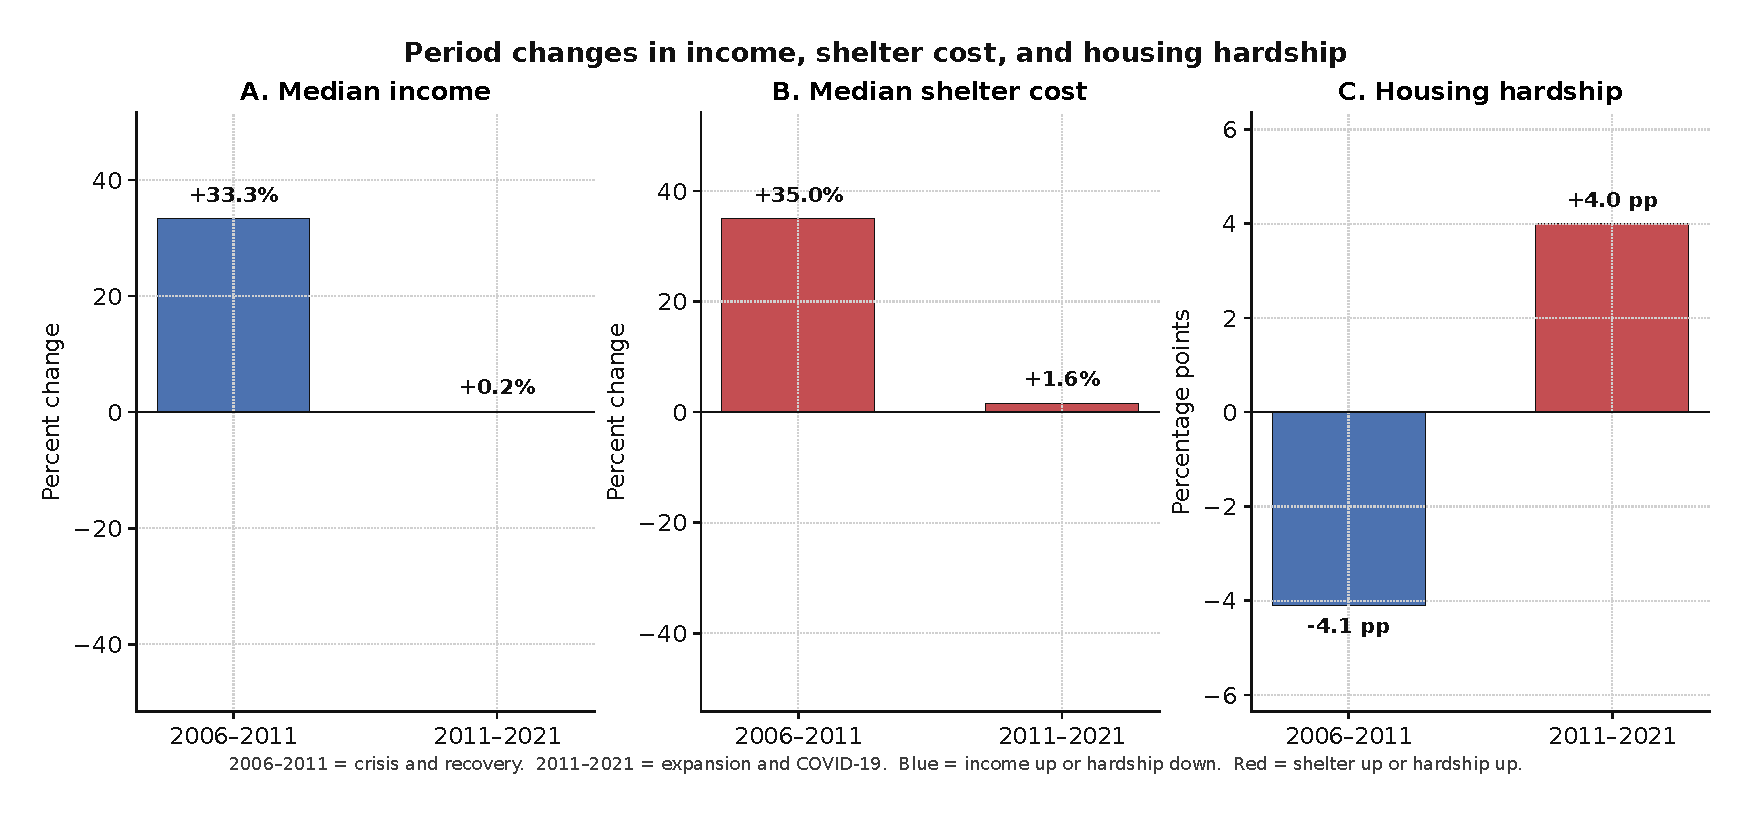
\includegraphics[width=0.98\textwidth]{fig02_period_comparison.pdf}
  \caption{Period comparison.
  Blue bars are income gains or hardship declines.
  Red bars are shelter-cost increases or hardship increases.
  The 2011--2021 expansion erased the 2006--2011 hardship gain.}
  \label{fig:periods}
\end{figure}

The crisis-and-recovery window (2006--2011) looks better on hardship ($-$4.1~pp) even though shelter rose fast, because real median income also rose 33.3\%.
The expansion-and-COVID window (2011--2021) looks worse: income was almost flat (+0.2\%), and hardship rose +4.0~pp.
A strong national economy did not repair leftover income.

\subsection{Owners versus renters}
\label{sec:tenure}

\begin{table}[htbp]
\centering
\caption{Housing hardship by tenure, 2011 and 2021}
\label{tab:tenure}
\small
\begin{tabular}{lrrr}
\toprule
Year & Owner hardship & Renter hardship & Gap \\
\midrule
2011 & 31.4\% & 40.4\% & 9.0 pp \\
2021 & 35.6\% & 43.6\% & 8.0 pp \\
Change & +4.2 pp & +3.2 pp & $-$1.0 pp \\
\bottomrule
\end{tabular}
\par\smallskip{\footnotesize Notes: Owner hardship is unavailable for 2006 because tenure coding in that PUMF file did not support a clean owner/renter split after cleaning. The gap narrowed because owners deteriorated toward renter rates, not because renters improved.}
\end{table}


\begin{figure}[htbp]
  \centering
  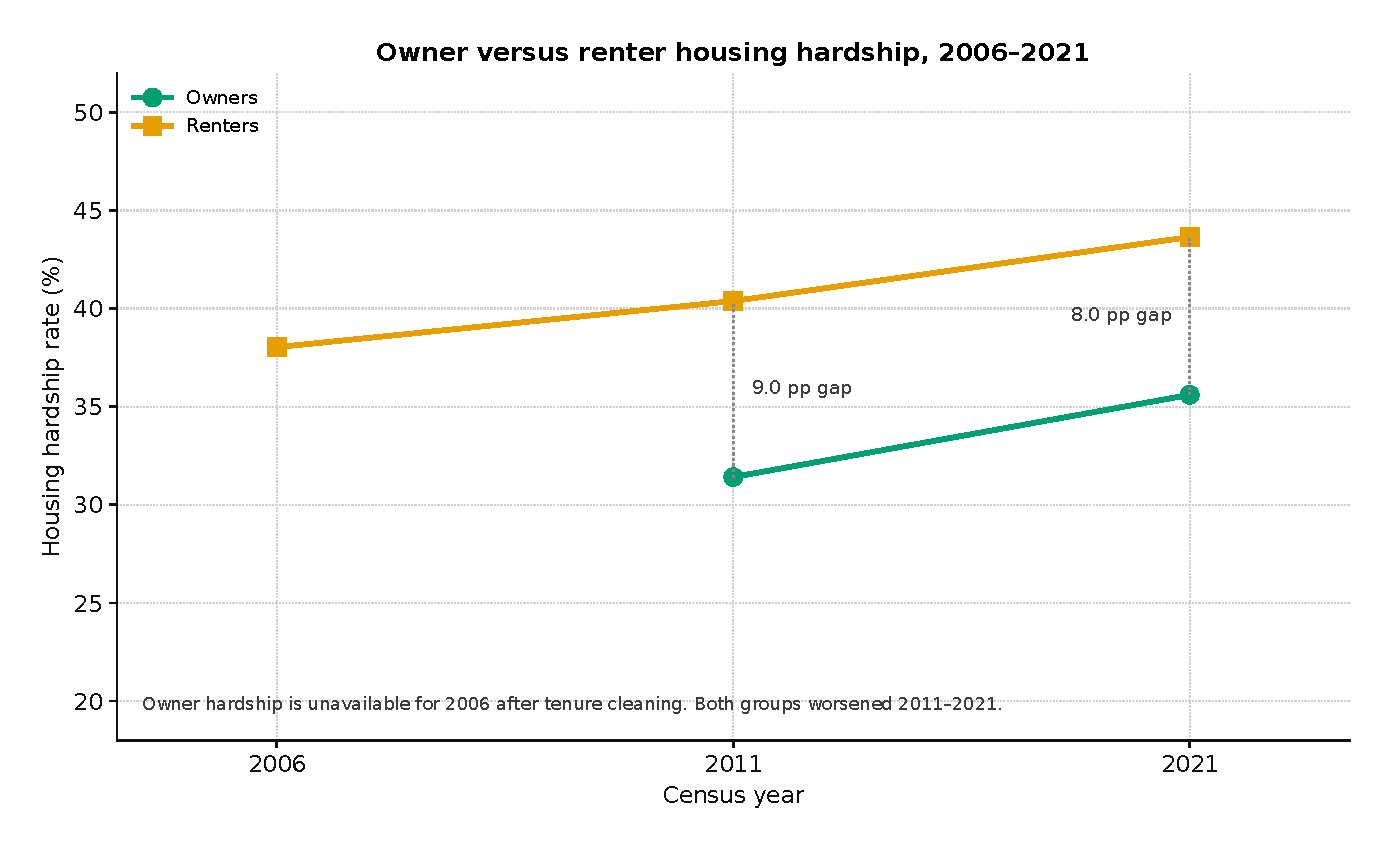
\includegraphics[width=0.88\textwidth]{fig03_tenure_divergence.pdf}
  \caption{Owner versus renter hardship.
  Renters stay higher.
  The gap narrowed from 9.0~pp to 8.0~pp because owners caught up, not because renters recovered.}
  \label{fig:tenure}
\end{figure}

Renters had higher hardship in both years with tenure data (40.4\% then 43.6\%).
Owner hardship rose from 31.4\% to 35.6\% (+4.2~pp, a 13.4\% relative increase).
Owning a home is not a guarantee of leftover-income security, especially with large mortgages, property tax, and repair bills.

\subsection{The indexed squeeze}
\label{sec:index}

\begin{table}[htbp]
\centering
\caption{Income versus shelter cost, indexed to 2006 = 100}
\label{tab:squeeze}
\small
\begin{tabular}{lrrr}
\toprule
Year & Income index & Shelter index & Gap \\
\midrule
2006 & 100.0 & 100.0 & 0.0 \\
2011 & 133.3 & 135.0 & 1.7 \\
2021 & 133.5 & 137.1 & 3.6 \\
\bottomrule
\end{tabular}
\par\smallskip{\footnotesize Notes: Index = (year median / 2006 median) $\times$ 100. Both series are in 2021 CAD. The 3.6-point 2021 gap equals about \$38 per month (\$456 per year) at the 2021 median.}
\end{table}


\begin{figure}[htbp]
  \centering
  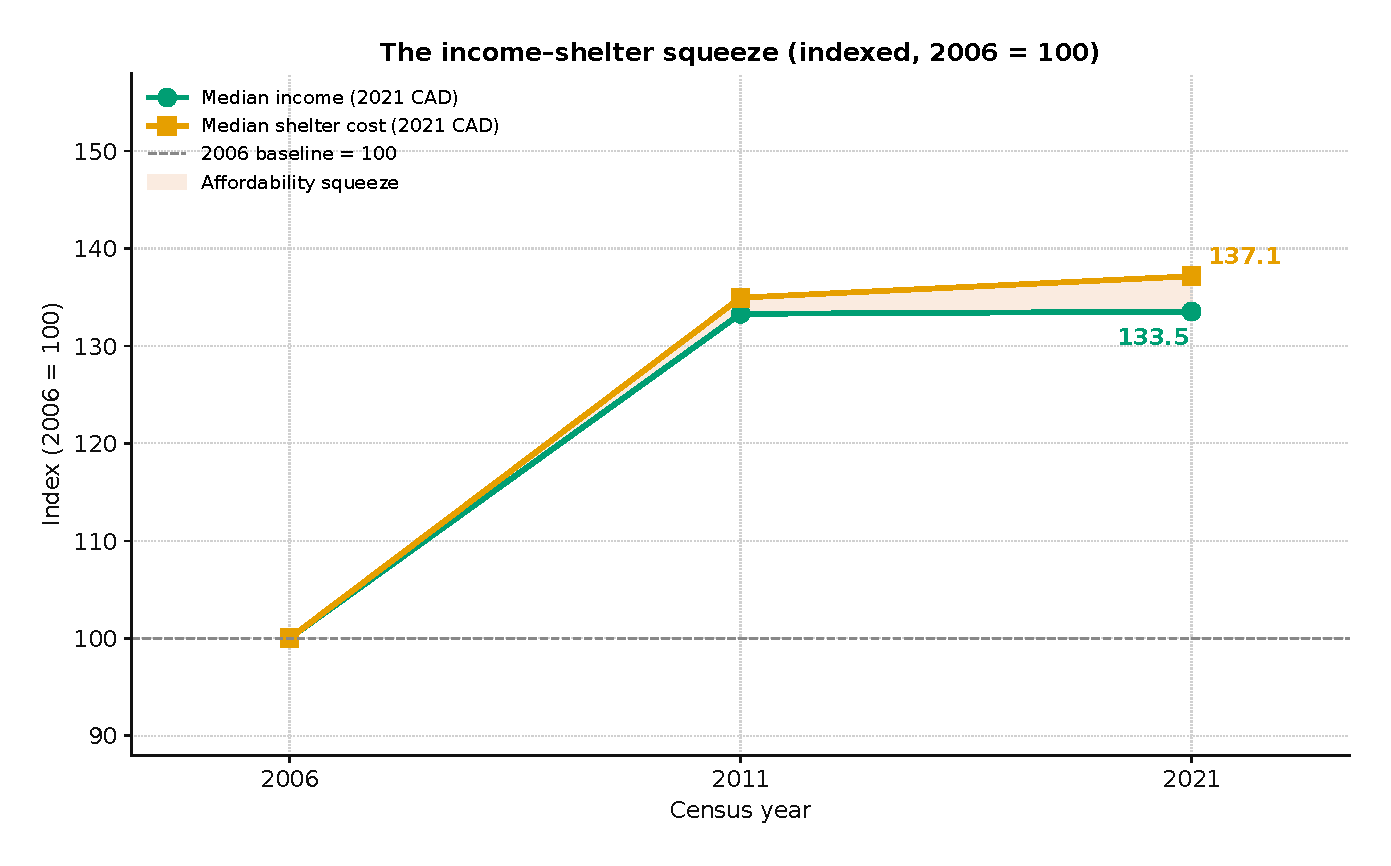
\includegraphics[width=0.88\textwidth]{fig04_income_shelter_squeeze.pdf}
  \caption{Income and shelter indexed to 2006 = 100.
  The shaded gap is the cumulative squeeze.
  By 2021 the shelter index (137.1) sits 3.6 points above the income index (133.5).}
  \label{fig:squeeze}
\end{figure}

The index chart makes the same 3.6-point gap visible without dollar scales.
Most of the real-income gain is already in place by 2011.
After that, shelter stays a little higher and leftover income erodes.

\subsection{Summary of the 15-year change}
\label{sec:sumres}

\begin{table}[htbp]
\centering
\caption{Summary statistics, 2006 versus 2021}
\label{tab:summary}
\small
\begin{tabular}{lrrr}
\toprule
Metric & 2006 & 2021 & 15-year change \\
\midrule
Median income (2021 CAD) & \$34,452 & \$46,000 & +33.5\% \\
Median monthly shelter & \$1,021 & \$1,400 & +37.1\% \\
STIR $>$ 30\% & 57.0\% & 50.8\% & $-$6.2 pp \\
Housing hardship & 38.0\% & 37.9\% & $-$0.1 pp \\
Renter hardship & 38.0\% & 43.6\% & +5.6 pp \\
Owner hardship & n/a & 35.6\% & n/a \\
\bottomrule
\end{tabular}
\par\smallskip{\footnotesize Notes: Owner hardship is not available for 2006. STIR improved while residual-income hardship did not, which is the central measurement result of this paper.}
\end{table}


\begin{figure}[htbp]
  \centering
  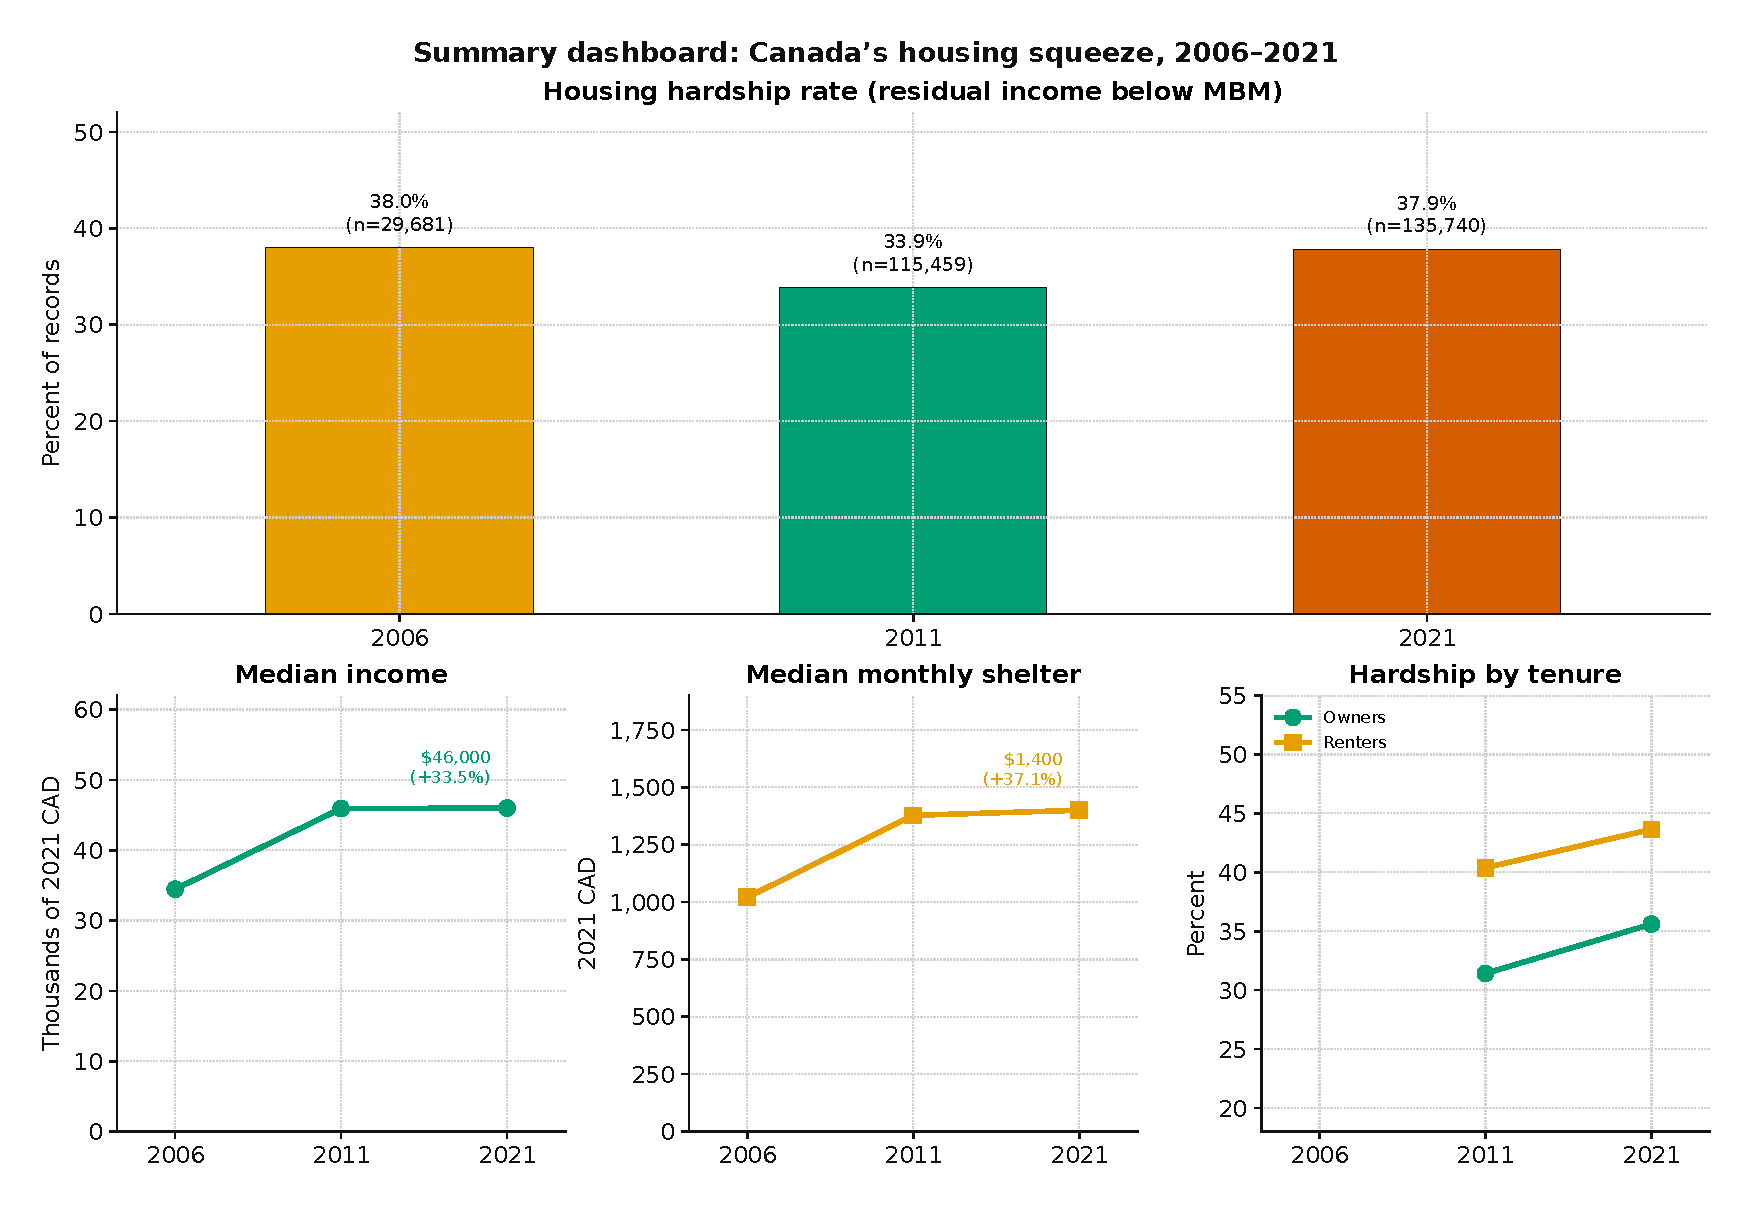
\includegraphics[width=\textwidth]{fig05_summary_dashboard.pdf}
  \caption{Summary dashboard.
  Hardship returns to the 2006 level.
  Median income and shelter both rise, but shelter rises more.
  Owner and renter hardship both increase after 2011.}
  \label{fig:dash}
\end{figure}

Four facts hold together:
\begin{enumerate}[leftmargin=1.6em]
  \item hardship stays near 38\%;
  \item shelter outruns income by 3.6~pp;
  \item STIR improves while leftover-income hardship does not;
  \item owners and renters both get worse after 2011.
\end{enumerate}

%% ====================================================================
\section{Discussion}
\label{sec:discussion}

\subsection{Structural, not cyclical}
\label{sec:structural}

If the crisis were only a recession leftover, hardship should have fallen a lot during the 2011--2019 expansion, low unemployment, and roughly 2\% average annual GDP growth.
It did the opposite: the 2011--2021 hardship rate rose 4.0~pp and ended at 37.9\%, almost the 2006 starting point (38.0\%).

Three patterns point to a built-in problem:
\begin{enumerate}[leftmargin=1.6em]
  \item hardship stays high through recovery;
  \item shelter grows faster than income in both periods we can measure cleanly;
  \item Conservative (2006--2015) and Liberal (2015--) federal governments both left the national residual-income rate near 38\%.
\end{enumerate}

\subsection{What the \$456 annual gap means}
\label{sec:gap}

For a 2021 median household (\$46,000 income; \$1,400 monthly shelter):
\begin{itemize}[leftmargin=1.4em]
  \item annual shelter = \$16,800;
  \item shelter if it had tracked income = about \$16,320;
  \item extra cost = \$480 a year (about \$38 a month).
\end{itemize}
That is 1.6\% of income and about 2.5\% of leftover income near the MBM line.
Over 15 years the same squeeze is on the order of \$3,600 in 2021 dollars---almost two months of median rent.
Low-income households, recent movers, and first-time buyers feel it first.

\subsection{Why owners are no longer safe}
\label{sec:owners}

The owner--renter gap shrank because owners deteriorated.
Likely channels include high mortgage debt taken on in hot markets, property tax and maintenance rising faster than wages, and ``house-rich, cash-poor'' seniors with equity but little leftover income.
Renter-only programs miss that group.

\subsection{Comparison with other research}
\label{sec:lit}

CMHC (2024) reports a much lower national hardship rate (7.8\% on 2020 data) than our 37.9\% in 2021 \cite{cmhc2024}.
The gap is expected.
CMHC uses the full Census, region-specific MBM lines, and family-size adjustments.
We use the 2.7\% PUMF sample and a single national adult MBM.
The \emph{level} is therefore not the headline.
The \emph{trend} is: the same method, applied to three waves, shows almost no 15-year improvement.

Walks and Twigge-Molecey (2023) show that Toronto and Vancouver diverge from other cities \cite{walks2023}.
A national PUMF average hides that geography.
Our national persistence result can still be true while some cities are much worse.

\subsection{Limitations}
\label{sec:limits}

\begin{enumerate}[leftmargin=1.6em]
  \item \textbf{Unweighted person-records.} Hierarchical PUMF files include a person weight (\texttt{WEIGHT}). This draft does not use it. Reported rates are shares of cleaned records, not official household population estimates.
  \item \textbf{Record type.} Each row is a person. After-tax income is the person field \texttt{TOTINC\_AT}, not the sum of household members. Shelter is a dwelling-level concept stored on person rows. Mixing those units can bias leftover income, especially in multi-person households.
  \item \textbf{2006 completeness.} Only 23.4\% of 2006 records survived cleaning, versus 99\%+ later. Pre-2016 cleaning kept \texttt{GROSRT} (rent) and dropped owners coded not-applicable. If missing 2006 records were poorer households, the 2006--2011 improvement is overstated.
  \item \textbf{No usable 2016 wave.} After the same missing-code rules, 9.4\% of the 2016-labelled file remained. We cannot split 2011--2016 recovery from 2016--2021 peak-and-COVID.
  \item \textbf{Census / NHS harmonization.} 2011 is the voluntary National Household Survey. Shelter names change from \texttt{GROSRT}/\texttt{OMP} to \texttt{SHELCO}. After-tax income missing codes are not identical across years. The three waves are comparable only after those caveats.
  \item \textbf{Simplified MBM.} A national single-adult leftover line understates hardship for large families and high-cost cities and overstates it for singles in cheaper regions. It is not the official 75F0002M table.
  \item \textbf{Cross-sections, not a panel.} We see snapshots, not the same households moving in and out of hardship.
  \item \textbf{No CMA split.} National rates hide Toronto/Vancouver versus Atlantic or Prairie patterns.
  \item \textbf{Broken PUMF means.} Hierarchical files inflate mean income when special codes remain. We therefore never interpret the mean; we use medians and percentiles.
\end{enumerate}

\subsection{Policy implications}
\label{sec:policy}

\textbf{Watch leftover income, not only STIR.}
STIR improved 6.2~pp while hardship did not.
A government that only tracks the 30\% rule will declare progress that leftover income does not show.

\textbf{Treat the problem as structural.}
Tax credits and small pilots did not move the 15-year hardship rate.
Supply (zoning, approvals, public housing), demand (empty-home and multi-property tax), and income support (rent supplements tied to MBM, wage growth) all have to move together.

\textbf{Help owners as well as renters.}
Owner hardship rose 4.2~pp.
Property-tax deferral and mortgage-renewal help belong in the same toolkit as rent supplements.

\textbf{Fix income stagnation.}
Real median income rose 0.2\% from 2011 to 2021.
Housing policy cannot succeed if typical pay is flat.

Other countries that treat housing as infrastructure rather than only as an asset---Vienna's social housing, Singapore's HDB flats, Finland's Housing First---have lower hardship.
Those are policy choices, not accidents of geography.

\subsection{Next steps for this project}
\label{sec:next}

A later paper can (i)~recover a clean 2016 file, (ii)~split results by CMA, (iii)~impute liquid assets from the Survey of Financial Security (the V3 model), and (iv)~run shock scenarios (rate resets, rent spikes, job loss).
Those steps add novelty.
They are not required to establish the 15-year residual-income trend.

%% ====================================================================
\section{Conclusion}
\label{sec:conclusion}

Using 777,707 Census records and a leftover-income test, we find:

\begin{enumerate}[leftmargin=1.6em]
  \item Housing hardship was 38.0\% in 2006 and 37.9\% in 2021. Fifteen years of growth did not fix it.
  \item Real shelter costs rose 37.1\%; real median income rose 33.5\%. The 3.6~pp gap is about \$456 a year at the 2021 median.
  \item The 30\% STIR rule improved. Residual-income hardship did not. Those two facts can be true at the same time.
  \item Owner hardship rose from 31.4\% to 35.6\% (2011--2021). Homeownership is not a shield.
  \item The 2011--2021 expansion, not the 2008-crisis window, is when leftover income got worse.
\end{enumerate}

The crisis is structural.
Another 15 years of the same tools will likely leave about 35--40\% of households without enough leftover income after housing.

%% ====================================================================
\begin{thebibliography}{9}

\bibitem{cmhc2024}
Canada Mortgage and Housing Corporation.
\newblock \emph{Revised Housing Hardship Methodology: Technical Documentation}.
\newblock CMHC Research Insights, 2024.

\bibitem{chs2024}
Statistics Canada.
\newblock \emph{Canadian Housing Survey: Housing Challenges and Experiences, 2024}.
\newblock Catalogue no.~46-28-0001.

\bibitem{hulchanski2020}
Hulchanski, J.~D., Walks, A., and Bourne, L.~S.
\newblock Canada's housing crisis: Dimensions, causes, and policy responses.
\newblock In T.~Bunting and P.~Filion (Eds.), \emph{Canadian Cities in Transition} (5th~ed., pp.~315--333).
\newblock Oxford University Press, 2020.

\bibitem{statcan2022pumf}
Statistics Canada.
\newblock \emph{Census 2021 Public Use Microdata File (PUMF): Hierarchical File Documentation}.
\newblock Catalogue no.~98M0002X, 2022.

\bibitem{statcan2021mbm}
Statistics Canada.
\newblock \emph{Market Basket Measure Thresholds, 2018-base}.
\newblock Catalogue no.~75F0002M, 2021.

\bibitem{walks2023}
Walks, A., and Twigge-Molecey, A.
\newblock Income mixing and housing affordability in Canadian cities.
\newblock \emph{Urban Studies}, 60(11), 2234--2254, 2023.

\end{thebibliography}

%% ====================================================================
\appendix
\section{Figure files (saved separately)}
\label{app:figures}

Each figure is exported as vector PDF, SVG, and 300~dpi PNG in the local \texttt{figures/} folder.
The manuscript includes the PDF files with \texttt{\textbackslash includegraphics}.

\begin{center}
\small
\begin{tabular}{lll}
\toprule
File stem & Figure & Content \\
\midrule
\texttt{fig01\_national\_trends.pdf} & Fig.~\ref{fig:national} & Income, shelter, STIR, hardship \\
\texttt{fig02\_period\_comparison.pdf} & Fig.~\ref{fig:periods} & 2006--2011 vs 2011--2021 \\
\texttt{fig03\_tenure\_divergence.pdf} & Fig.~\ref{fig:tenure} & Owners vs renters \\
\texttt{fig04\_income\_shelter\_squeeze.pdf} & Fig.~\ref{fig:squeeze} & Indexed squeeze \\
\texttt{fig05\_summary\_dashboard.pdf} & Fig.~\ref{fig:dash} & Four-panel summary \\
\bottomrule
\end{tabular}
\end{center}

\section{Table files (saved separately)}
\label{app:tables}

Each table exists as CSV (for spreadsheets) and as a \texttt{.tex} snippet (for \texttt{\textbackslash input}).
Files live in the local \texttt{tables/} folder.

\begin{center}
\small
\begin{tabular}{lll}
\toprule
CSV / TeX stem & Table & Content \\
\midrule
\texttt{table01\_sample\_characteristics} & Table~\ref{tab:sample} & Sample and medians \\
\texttt{table02\_tenure\_hardship} & Table~\ref{tab:tenure} & Owner vs renter \\
\texttt{table03\_indexed\_squeeze} & Table~\ref{tab:squeeze} & 2006 = 100 indexes \\
\texttt{table04\_summary\_2006\_2021} & Table~\ref{tab:summary} & 15-year summary \\
\texttt{table05\_period\_changes} & Table~\ref{tab:periods} & Period changes \\
\bottomrule
\end{tabular}
\end{center}

To rebuild figures and tables from the JSON results file:

\begin{verbatim}
python3 papers/paper1_highschool/generate_figures_tables.py
\end{verbatim}

To compile this paper:

\begin{verbatim}
cd papers/paper1_highschool
pdflatex paper1_highschool.tex
pdflatex paper1_highschool.tex
\end{verbatim}

\section{How this version differs from Drafts 1.0 and 2.0}
\label{app:diff}

Draft 1.0 used story headings and did not ship separate figure or table files.
Draft 2.0 restored IMRAD headings and added figures, but the Drive JPEG previews clipped Figure~1 and Figure~5, used a bright-green Figure~2 fill, and placed the 2021 tick too far right on a linear time axis.
Draft 3.0 rebuilds all five figures from \texttt{generate\_figures\_tables.py} as PDF, SVG, and 300~dpi PNG on a white background with equally spaced year labels.
The plotted numbers are unchanged.
The methods and limitations sections now state the unresolved issues: unweighted person-records, person versus household units, the simplified MBM line, 2006/2016 exclusions, and Census/NHS shelter-variable harmonization.

\end{document}
